\section{Satellite Configuration}
\definecolor{blue}{rgb}{0.2,0.5,0.8}

\begin{longtable}{| l | r | r | r |}
	\hline
	\rowcolor[gray]{0.80}	\textbf{System}& \textbf{Weight/unit (g)} & \textbf{Sizes (mm)} & \textbf{N. of units}\\
	\hline
	\hline
	\endfirsthead
	
	
	\rowcolor[gray]{0.85} \textbf{STRUCTURE AND MECHANICS} & & & \\ \hline
	
	~Structure & 304.3 & 100 x 100 x 300& 1 \\
	~Thermal protection & 38 & Covers all & 1\\
	\hline 
	\rowcolor[gray]{0.95} \textbf{Total} & 342.3 & &  \\
	\hline \hline
	
	\rowcolor[gray]{0.85} \textbf{ELECTRIC POWER SYSTEM} & & & \\\hline
	
	~Solar arrays & 175 & 98 x 83 x 8.50 & 4 \\
	~Batteries & 155 & 90 x 63 x 12.02 & 2 \\
	~Power management & 126 & 92.0 x 88.9 x 20.5 & 1 \\
	\hline
	\rowcolor[gray]{0.95} \textbf{Total} & 1136 &  &  \\
	\hline \hline
	
	\rowcolor[gray]{0.85} \textbf{PAYLOAD} & & & \\ \hline
	
	~Patch antenna & 30 & 90 x 90 x4.35& 8 \\
	~Transceiver inter-satellite & 16.4 & 65 x 40 x 6.5 & 3 \\
	~Transceiver space to ground & 101.5 & 86 x 86 x 45 & 1 \\
	~Data handling system & 28.3 & 65 x 40 x 6.5 & 1\\
	~Antenna Deployable & 83 & 100 x 83 x 6.5 &1\\
	\hline
	\rowcolor[gray]{0.95} \textbf{Total} & 502 &  & \\
	\hline \hline \hline
	
	\rowcolor[gray]{0.85} \textbf{AOCDS} & & &\\ \hline
	
	~Thruster & 1500 & 90 x 90 x 95 & 1 \\
	~ADACS & 506 & 90 x 90 x 58 & 1 \\
	\hline
	\rowcolor[gray]{0.95} \textbf{Total} & 2006 &  & \\
	\hline \hline
	
	\rowcolor[gray]{0.9} \textbf{TOTAL ESTIMATION} & \textbf{3986.3} & & \\ \hline
	
	
\end{longtable} 

\textbf{STRUCTURE}
\begin{longtable}{| l | c  }
	\hline
	\rowcolor[gray]{0.80}	\textbf{Brand and model} &  \textbf{Features}     \\
	\hline
	\endfirsthead
	
	\rowcolor[gray]{0.85} \textbf{Structure} &  \\
	~ISIS 3U structure & \makecell{Low mass (304.3g) \\ Highly compatible \\ High temperature range}\\
	\hline
	\rowcolor[gray]{0.85} \textbf{Thermal protection} &  \\
	~Dunmore Aerospace Satkit & \makecell{Lightweight \\ Durability \\ Made for small satellites}\\
	\hline
		
	\caption{Estructure characteristics}
	\label{structureoptions}
\end{longtable}

\textbf{EPS}
\begin{longtable}{| l | c | }
	\hline
	\rowcolor[gray]{0.80}	\textbf{Brand and model} &  \textbf{Features}     \\
	\hline
	\endfirsthead
	
	\rowcolor[gray]{0.85} \textbf{Solar arrays} &  \\
	~EXA-Agencia Espacial Ecuatoriana & \makecell{Total power of 67.2W (4units)\\ Mass of 270g (p.unit) \\ Included thermal protection \\At least 4 years lifetime}  \\
	\hline
	\rowcolor[gray]{0.85} \textbf{Power management} &   \\
	~Gomspace NanoPower P60 & \makecell{Mass of 176g \\ 9x configurable outputs \\ 6x inputs per module \\ EMI shielding \\ High temperature range} \\
	\hline
	\rowcolor[gray]{0.85} \textbf{Batteries} &   \\
	~EXA-Agencia Espacial Ecuatoriana & \makecell{Total capacity of 106.4Wh (2u)\\ Automatic heat regulation \\ Highly stackable \\ Total mass of 155g} \\
	\hline
	
	\caption{Electric Power System}
	\label{epsoptions}
\end{longtable}

\textbf{Propulsion System}
\begin{longtable}{| l | r |}
	
	\hline
	
	\rowcolor[gray]{0.60} \multicolumn{2}{|c|}{\textbf{Thruster BGT-X5}} \\
	
	\hline
	
	\hline
	\rowcolor[gray]{0.75}	\textbf{PARAMETERS} &  \textbf{VALUE}   \\
	\hline
	
	\cellcolor[gray]{0.85} \textbf{Total thruster power} & 20 W  \\
	\cellcolor[gray]{0.85} \textbf{Thrust} & 0.5 N \\
	\cellcolor[gray]{0.85} \textbf{Specific impulse} & 225 s \\
	\cellcolor[gray]{0.85} \textbf{Thruster Mass} & 1500 g \\
	\cellcolor[gray]{0.85} \textbf{Input voltage} & 12 V \\
	\cellcolor[gray]{0.85} \textbf{Delta V} & 146 m/s \\
	\hline
	\caption{Main features of BGT-X5}
	\label{thrusterfinal}
\end{longtable}

\textbf{ADOCS}
\begin{longtable}{| l | c |}
	
	\hline
	\rowcolor[gray]{0.60} \multicolumn{2}{|c|}{\textbf{ADACS}} \\
	\hline
	
	\hline
	\rowcolor[gray]{0.75}	\textbf{Features} &  \textbf{CUBE ADCS} \\
	\hline
	
	\cellcolor[gray]{0.85} \textbf{Power} &\makecell{3.3/5 VDC\\ Peak: 7.045W }  \\ 	\hline
	\cellcolor[gray]{0.85} \textbf{Mass} & 506 g\\ \hline
	\cellcolor[gray]{0.85} \textbf{Size} & 90 x 90 x 58 mm \\ \hline
	\cellcolor[gray]{0.85} \textbf{Sensors} & \makecell{3-Axis Gyro\\Fine Sun \& Earth sensor \\ Magnetometer\\10x Coarse Sun Sensors \\Star tracker(optional)}\\ 	\hline
	\cellcolor[gray]{0.85} \textbf{Actuators} &  \makecell{3 reactions wheels\\2 torque rods}\\ 	\hline
	\cellcolor[gray]{0.85} \textbf{Computer} &\makecell{4-48 MHz\\ full ADCS + OBC}   \\ \hline
	\cellcolor[gray]{0.85} \textbf{Control Board} & \makecell{Works as OBC\\included}\\
	\hline
	
	\caption{Main ADACS features}
	\label{ADACS}
	
\end{longtable}
\textbf{Payload}
\begin{longtable}{| l | r |}
	
	\hline
	\rowcolor[gray]{0.60} \multicolumn{2}{|c|}{\textbf{Patch antenna AntDevCo}} \\
	%\rowcolor[gray]{0.60}	\multicolumn{2}{|l|}{\textbf{Patch antenna}} \\
	\hline
	
	\hline
	\rowcolor[gray]{0.75}	\textbf{Features} &  \textbf{Value}   \\
	\hline
	
	\cellcolor[gray]{0.85} \textbf{Bands} & L,S,C,X  \\
	\cellcolor[gray]{0.85} \textbf{Frequency range} & 1-12 GHz  \\
	\cellcolor[gray]{0.85} \textbf{Bandwidth} & 20 MHz \\
	\cellcolor[gray]{0.85} \textbf{Gain} & 6 dBi  \\
	\cellcolor[gray]{0.85} \textbf{Polarization} & Circular \\
	\cellcolor[gray]{0.85} \textbf{Maximum power consumption} & 10 W \\
	\cellcolor[gray]{0.85} \textbf{Impedance} & 50 Ohms \\
	\cellcolor[gray]{0.85} \textbf{Operational temperature range} & -65ºC to +100ºC \\
	\cellcolor[gray]{0.85} \textbf{Mass} & <250 grams \\
	\hline
	\caption{Main features of the patch antenna}
	\label{patchantenna}
\end{longtable}
\begin{longtable}{| l | r | r |}
	
	\hline
	\rowcolor[gray]{0.60} \multicolumn{3}{|c|}{\textbf{Inter-satellite comm.(S band)}} \\
	\hline
	
	\hline
	\rowcolor[gray]{0.75}	\textbf{Features} &  \textbf{NanoCom TR-600}  \\
	\hline
	
	\cellcolor[gray]{0.85} \textbf{Band} & 70 - 6000 MHz \\
	\cellcolor[gray]{0.85} \textbf{Bandwidth} & 0.2 - 56 MHz\\
	\cellcolor[gray]{0.85} \textbf{Vcc} & 3.3V \\
	\cellcolor[gray]{0.85} \textbf{Max. Power consumption} & 14W\\
	\cellcolor[gray]{0.85} \textbf{Dimensions} & 65 x 40 x 6.5 mm \\
	\cellcolor[gray]{0.85} \textbf{Operational temperature range} & -40ºC to +85ºC\\
	\cellcolor[gray]{0.85} \textbf{Mass} & 16,4 grams \\
	\hline
	
	\caption{Main inter-satellite communication transceiver features}
	\label{TransceiversSband}
	
\end{longtable}
\begin{longtable}{| l | r | r |}
	
	\hline
	\rowcolor[gray]{0.60} \multicolumn{3}{|c|}{\textbf{Space to Ground comm.(X band)}} \\
	\hline
	
	\hline
	\rowcolor[gray]{0.75}	\textbf{Features} &  \textbf{SWIFT-XTS}  \\
	\hline
	
	\cellcolor[gray]{0.85} \textbf{Band} & 7 - 9 GHz  \\
	\cellcolor[gray]{0.85} \textbf{Bandwidth} & 10 - >100 MHz\\
	\cellcolor[gray]{0.85} \textbf{Vcc} & 3.3V\\
	\cellcolor[gray]{0.85} \textbf{Max. Power consumption} & 12W\\
	\cellcolor[gray]{0.85} \textbf{Dimensions} & 86 x 86 x 45mm \\
	\cellcolor[gray]{0.85} \textbf{Operational temperature range} & -40ºC to +85ºC\\
	\cellcolor[gray]{0.85} \textbf{Mass} & 350 grams \\
	\hline
	
	\caption{Main space to ground communication transceiver features}
	\label{TransceiversXband}
	
\end{longtable}

\begin{longtable}{| l | r | r |}
	
	\hline
	\rowcolor[gray]{0.60} \multicolumn{3}{|c|}{\textbf{PDHS computers options}}\\
	\hline
	
	\hline
	\rowcolor[gray]{0.75}	\textbf{Features} &  \textbf{NanoMind Z7000} \\
	\hline
	
	\cellcolor[gray]{0.85} \textbf{Operating System} & Linux \\
	\cellcolor[gray]{0.85} \textbf{Storage} & 4GB to 32 GB\\
	\cellcolor[gray]{0.85} \textbf{Processor} & MPCoreA9 667 MHz\\
	\cellcolor[gray]{0.85} \textbf{Vcc} & 3.3V \\
	\cellcolor[gray]{0.85} \textbf{Max. Power consumption} & 30W\\
	\cellcolor[gray]{0.85} \textbf{Dimensions} & 65 x 40 x 6.5mm \\
	\cellcolor[gray]{0.85} \textbf{Operational temperature range} & -40ºC to +85ºC \\
	\cellcolor[gray]{0.85} \textbf{Mass} & 28.3 grams \\
	\hline
	
	\caption{Main PDHS computer features}
	\label{computers}
	
\end{longtable}

\textbf{LINK} 
\paragraph{} Payload communication capabilities. Depending onthe Bandwidth selected a Sensitivity, S, is imposed by \ref{SvsB}. Then with this fixed power is possible to obtain the range of communication from Figure\ref{friis}.
\begin{figure}[h]
	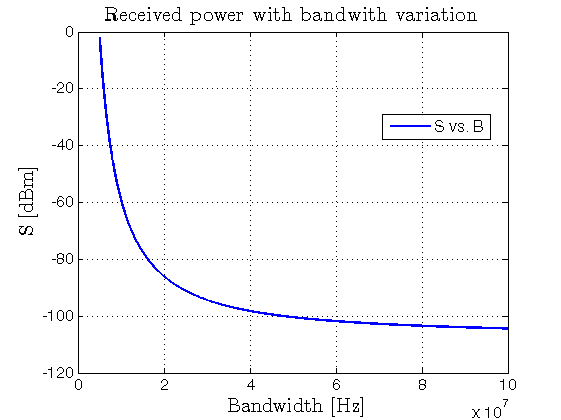
\includegraphics[scale=0.9]{./sections/SatelliteConfiguration/SvsB}
	\centering
	\caption{Sensibility change along Bandwidth variation}
	\label{SvsB}
\end{figure}
\begin{figure}[h]
	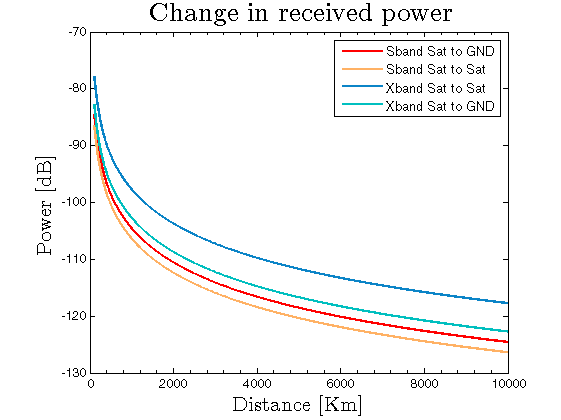
\includegraphics[scale=0.9]{./sections/SatelliteConfiguration/friisCases}
	\centering
	\caption{Received power with distance variation}
	\label{friis}
\end{figure}
\clearpage
FALTA JUNTAR UN ESQUEMA THE RELACIÓN ENTRE COMPONENTES
%\input{../sections/SatelliteConfiguration/Visio-ESQUEMA_ASTREASAT.pdf}
%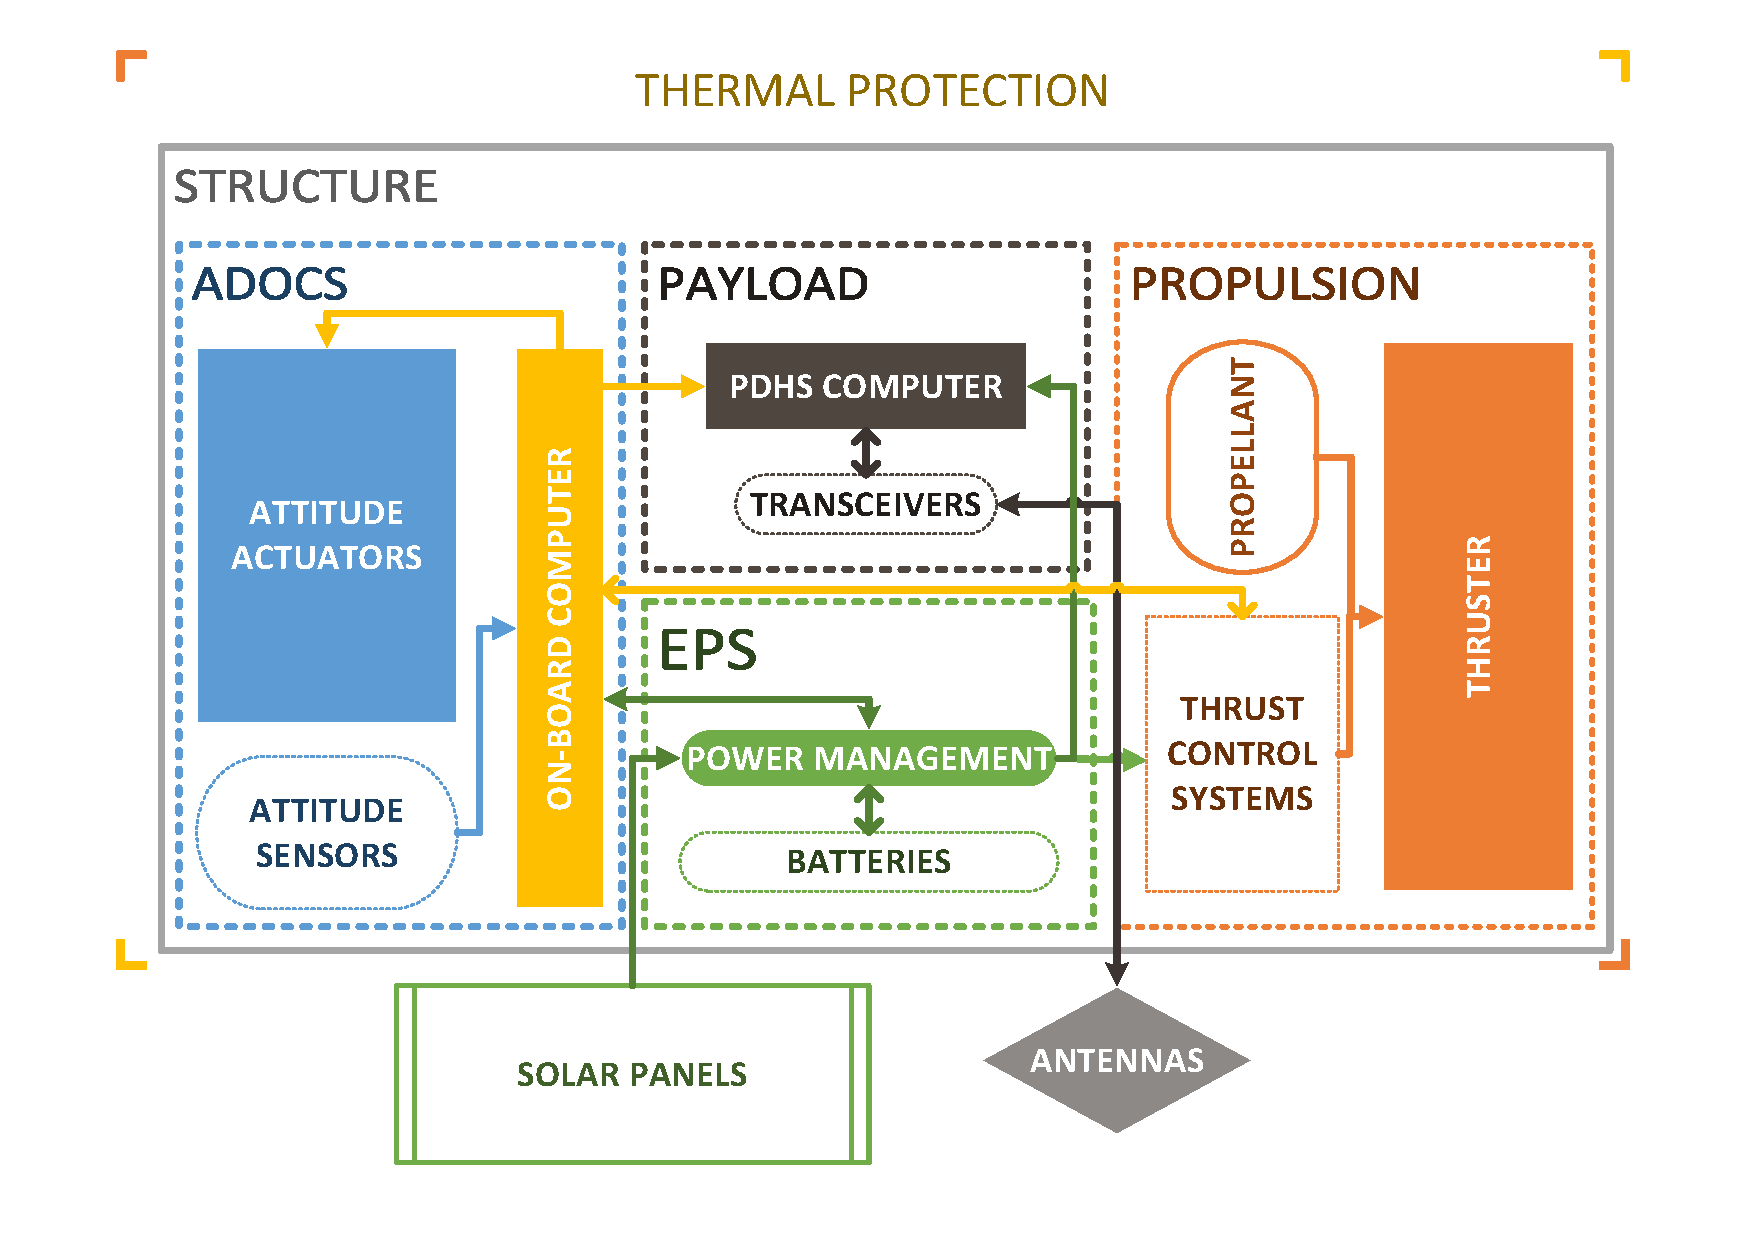
\includepdf{../sections/SatelliteConfiguration/Visio-ESQUEMA_ASTREASAT.pdf}

